
\documentclass[11pt,a4paper,openany]{report}
\usepackage[T1]{fontenc}
\usepackage[utf8]{inputenc}
\usepackage{lmodern}
\usepackage{microtype}
\usepackage{amsmath,amssymb,amsthm,mathtools,bm}
\usepackage{booktabs,array,longtable,tabularx}
\usepackage{xcolor}
\usepackage[margin=22mm,headheight=23pt]{geometry}
\usepackage{enumitem}
\usepackage{fancyhdr}
\usepackage{fancyvrb}
\usepackage{graphicx}
\usepackage{url}
\usepackage{xurl}
\usepackage{hyperref}
\definecolor{finblue}{HTML}{1F5A99}
\definecolor{fingreen}{HTML}{19733A}
\definecolor{finorange}{HTML}{D55E00}
\definecolor{finred}{HTML}{A61B1B}
\definecolor{finviolet}{HTML}{6A3D9A}
\definecolor{fingray}{HTML}{4D4D4D}

\hypersetup{
  unicode=true,
  colorlinks=true,
  linkcolor=finblue,
  citecolor=fingreen,
  urlcolor=finblue,
  pdftitle={FIN Research Programs P323--P336},
  pdfauthor={Krzysztof Żuchowski},
  pdfsubject={Exact resource certificates, refreeze provenance, and operational transfer boundaries},
  pdfkeywords={FIN, signed moment, Jordan measure, phase lattice, refreeze provenance, exact spectral chambers, diamond distance, photonic transfer, resource independence}
}
\pagestyle{fancy}
\fancyhf{}
\fancyhead[L]{\small FIN Programs P323--P336}
\fancyhead[R]{\small Release 10.29}
\fancyfoot[C]{\thepage}

\setlength{\parindent}{0pt}
\setlength{\parskip}{0.55em}
\setlist{nosep,leftmargin=2em}
\setcounter{tocdepth}{2}
\setcounter{secnumdepth}{3}
\emergencystretch=3em
\newcommand{\one}{\bm 1}
\newcommand{\C}{\mathbb C}
\newcommand{\R}{\mathbb R}
\newcommand{\Z}{\mathbb Z}
\newcommand{\statusProven}{\textcolor{fingreen}{[Proven]}}
\newcommand{\statusStrong}{\textcolor{finblue}{[Strong evidence]}}
\newcommand{\statusModerate}{\textcolor{finviolet}{[Moderate evidence]}}
\newcommand{\statusWeak}{\textcolor{fingray}{[Weak evidence]}}
\newcommand{\statusSpeculative}{\textcolor{finorange}{[Speculative]}}
\newcommand{\statusRefuted}{\textcolor{finred}{[Refuted]}}

\begin{document}
\hypersetup{pageanchor=false}
\begin{titlepage}
\centering
\vspace*{7mm}
{\Large\bfseries FIN --- Release 10.29\par}
\vspace{9mm}
{\Huge\bfseries Research Programs P323--P336\par}
\vspace{6mm}
{\Large Exact resource certificates,\\
refreeze provenance,\\
and operational transfer boundaries\par}
\vspace{13mm}
{\Large Krzysztof \.Zuchowski\par}
\vspace{2mm}
{\normalsize Independent Researcher --- Fractal Information Theory Project\par}
\vspace{2mm}
{\normalsize ORCID:
\href{https://orcid.org/0009-0002-0909-3613}{0009-0002-0909-3613}\par}
\vspace{7mm}
{\large 30 July 2026\par}
{\normalsize Publication --- Preprint; Version 1.0.0\par}
\vfill
\begin{minipage}{0.92\textwidth}
\small
\textbf{Central result.}
A matching signed-measure/dual-polynomial certificate fixes the continuum
seven-moment negative path resource at
\(\mathcal N_{\rm path}=0.406706334692258\ldots\).

\medskip
\textbf{Phase provenance.}
The exact strict phase unit \(1/4000\) is the gcd lattice unit generated by
the QW-2030 center and QW-2038 grid steps.  This is a procedural provenance
theorem, not an internal physical source theorem.

\medskip
\textbf{Repository.}
\url{https://github.com/hyconiek/Fractal-Nadsoliton-Theory}

\textbf{License.} CC BY 4.0.
\end{minipage}
\vfill
\end{titlepage}
\hypersetup{pageanchor=true}
\pagenumbering{roman}
\chapter*{Publication statement}
\addcontentsline{toc}{chapter}{Publication statement}
This monograph reports all executed Programs P323--P336 and recommends
Programs P337--P350.  Mathematical proof, high-precision evaluation,
target-dependent construction, synthetic design, conditional axiom package,
and missing external evidence remain separate.  The legacy/strict split,
QW-2191, dimensional-source, role-transfer, laboratory, \(L_{\rm total}\),
Standard-Model/gravity, and Theory-of-Everything boundaries are preserved.

\tableofcontents
\clearpage
\pagenumbering{arabic}

\chapter*{Confidence convention}
\addcontentsline{toc}{chapter}{Confidence convention}

\begin{itemize}
\item 
\textbf{\statusProven{}}: an analytic or finite exact implication is supplied.

\item 
\textbf{\statusStrong{}}: deterministic or replicated computation supports the claim inside a declared model.

\item 
\textbf{\statusModerate{}}: the result is robust in a narrower design class.

\item 
\textbf{\statusSpeculative{}}: a mechanism is proposed without decisive evidence.

\item 
\textbf{\statusRefuted{}}: the declared hypothesis class fails.

\item 
\textbf{[Blocked by external evidence]}: the result requires a genuine outside record, apparatus, or custody relation.

\end{itemize}

\section{Separation of proof layers}

Each program distinguishes:

\begin{enumerate}
\item 
a theorem valid for a mathematical class;

\item 
an evaluation for the frozen FIN numbers;

\item 
a synthetic design calculation;

\item 
an external experimental statement.

\end{enumerate}

Numerical agreement cannot move a claim upward in this hierarchy.

\section{Reproducibility}

The deterministic runner uses seed

\[
20260803.
\]

It produces machine-readable JSON, twelve detailed CSV tables, seven figures, and a Lean 4.28 source.  External programs P330 and P336 are admission audits: the runner cannot generate their success conditions.

\chapter{P323 --- Continuum signed-moment duality}

\section{Primal problem}

Let

\[
h_k=\frac1{1+k^{9/5}},
\qquad k=0,\dots,6.
\]

Among signed Borel measures

\[
\mu=\mu_+-\mu_-
\]

on \([0,1]\) satisfying

\[
\int_0^1 x^k\,d\mu(x)=h_k,
\qquad k=0,\dots,6,
\]

minimize the negative Jordan mass

\[
\mathcal N(\mu)=\mu_-([0,1]).
\]

The shifted moments \(h_1,\ldots,h_6\) determine a three-node Gaussian rule. Let

\[
g(x)=x^3+c_2x^2+c_1x+c_0
\]

be orthogonal to \(1,x,x^2\) for the shifted moment functional.  Numerically,

\[
\begin{aligned}
c_0&=-0.11092397533402947096\ldots,\\
c_1&= \phantom{-}0.79990303366942818900\ldots,\\
c_2&=-1.63824233917926923454\ldots.
\end{aligned}
\]

Its roots are

\[
\begin{aligned}
r_1&=0.23727834187306726370\ldots,\\
r_2&=0.54819801698629973919\ldots,\\
r_3&=0.85276598031990223166\ldots.
\end{aligned}
\]

The positive weights are

\[
\begin{aligned}
u_1&=0.94183420338052919615\ldots,\\
u_2&=0.39368551953570941935\ldots,\\
u_3&=0.07118661177601972793\ldots.
\end{aligned}
\]

Define

\[
\mu_*=
\sum_{j=1}^{3}u_j\delta_{r_j}
-\mathcal N_*\delta_0,
\qquad
\mathcal N_*=\sum_j u_j-1.
\]

Then

\[
\mathcal N_*
=0.40670633469225834343\ldots
\]

and all seven moment residuals are below \(3.1\times10^{-92}\) in the 90-digit computation.

\section{Dual problem}

For any polynomial

\[
-1\le p(x)\le0
\quad\text{on}\quad[0,1],
\]

and any feasible signed measure,

\[
\sum_{k=0}^{6}p_kh_k
=\int p\,d\mu
\le\mu_-([0,1]).
\]

This is weak duality.

Set

\[
q(x)=\frac{g(x)}{g(0)},
\qquad
p_*(x)=-q(x)^2.
\]

The polynomial \(p_*\) vanishes at all three positive atoms and equals \(-1\) at the negative atom \(x=0\).  Its coefficients in ascending order are

\[
\begin{aligned}
(&-1,\,
14.4225453741745,\,
-81.5405646086897,\,
231.037739077899,\\
&-348.146892117430,\,
266.291491557255,\,
-81.2735348088558).
\end{aligned}
\]

The two internal critical points of \(q\) have squared magnitudes approximately \(0.01060\) and \(0.00987\), while \(q(1)^2\approx0.20922\).  Thus \(q(x)^2\le1\) on \([0,1]\), so \(p_*\) is dual-feasible.

Finally,

\[
\sum_{k=0}^{6}(p_*)_kh_k
=0.40670633469225834343\ldots
=\mathcal N_*.
\]

Matching primal and dual values prove optimality.

\section{Interpretation}

The strict attenuation cannot be generated by a positive distribution of exponential distance scales.  Within this seven-moment representation, the minimum signed resource is approximately \(0.4067063\), not merely nonzero.

This does \textbf{not} prove:

\begin{itemize}
\item 
a quantum quasiprobability;

\item 
negative thermodynamic entropy;

\item 
physical information destruction;

\item 
an open-system reservoir;

\item 
a unique microscopic path model.

\end{itemize}

\begin{figure}[htbp]
\centering
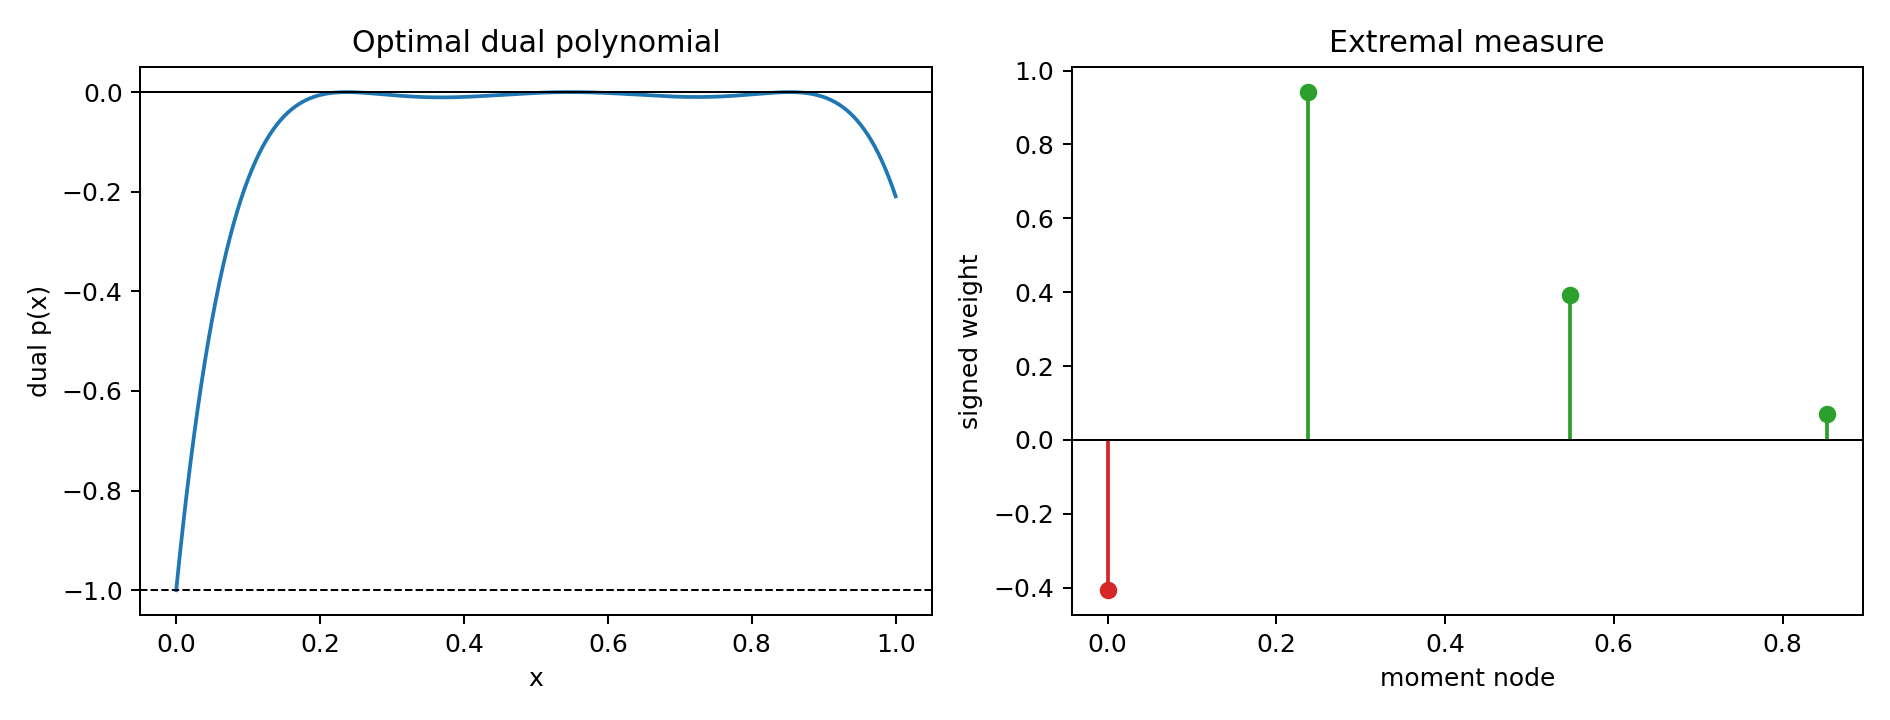
\includegraphics[width=0.97\textwidth]{FIN_Programs_323_336_Figures/p323_continuum_extremizer.png}
\caption{The matching continuum signed-measure and dual-polynomial extremizers.}
\end{figure}

\chapter{P324--P325 --- Source independence and phase provenance}

\section{P324: completion fibers}

Let \(A_L\) be the repaired positive legacy operator.  Consider a deterministic completion rule

\[
F:A_L\longmapsto A_T.
\]

Three distinct positive radial target operators were constructed on the same carrier and with exactly the same input \(A_L\):

\begin{enumerate}
\item 
the frozen strict target;

\item 
an alternative with \((\omega,\phi,\beta,\eta)
   =(0.20175,0.11250,0.92,1.7)\);

\item 
an alternative with \((0.16975,0.06250,0.84,1.6)\).

\end{enumerate}

For each target \(A_T\), the block operator

\[
\mathcal P_T=
\begin{pmatrix}
A_L & A_L^{1/2}A_T^{1/2}\\
A_T^{1/2}A_L^{1/2} & A_T
\end{pmatrix}
\]

is positive up to numerical roundoff and has cross support.  But the cross block explicitly reads \(A_T\).

Therefore:

\[
A_{T,1}\ne A_{T,2}
\quad\Longrightarrow\quad
\neg\bigl(
F(A_L)=A_{T,1}
\ \wedge\
F(A_L)=A_{T,2}
\bigr).
\]

The common-parent construction is a representation theorem, not a source-independent generation theorem.

The newly defined object O76 is the \textbf{completion fiber}

\[
\mathfrak F(A_L)=
\{A_T:\ A_T\text{ satisfies the declared target-side admissibility rules}\}.
\]

A source law must select one point of this fiber without reading the chosen target in advance.

\section{P325: exact lattice genealogy}

The QW-2030 upstream center was

\[
\omega_0=\frac{187}{800},
\qquad
\phi_0=-\frac{11}{80}.
\]

The QW-2038 grids used exact decimal steps

\[
\Delta\omega=0.016=\frac{2}{125},
\qquad
\Delta\phi=0.05=\frac1{20}.
\]

The selected row is obtained by the grid indices \((-3,+6)\):

\[
\omega_*=\omega_0-3\Delta\omega
=\frac{743}{4000},
\]

\[
\phi_*=\phi_0+6\Delta\phi
=\frac{13}{80}
=\frac{650}{4000}.
\]

The additive subgroup of \(\mathbb Q\) generated by the two centers and two steps is

\[
\left\langle
\frac{187}{800},
\frac{2}{125},
-\frac{11}{80},
\frac1{20}
\right\rangle_{\mathbb Z}
=
\frac1{4000}\mathbb Z.
\]

Hence the generator

\[
r=e^{i/4000}
\]

is minimal for the \textbf{procedural refreeze lattice}.

\section{Falsification of an internal-source reading}

The provenance chain uses:

\begin{itemize}
\item 
supplied upstream center values;

\item 
investigator-chosen grid widths and step counts;

\item 
a mass/\allowbreak{}flavor/\allowbreak{}GW objective;

\item 
threshold gates;

\item 
selection of the best passing row.

\end{itemize}

This is a real derivation of the selected grid coordinate from a declared search protocol.  It is not a derivation of the coordinate from the informational nadsoliton alone.

Accordingly:

\begin{center}
\begingroup\small
\setlength{\tabcolsep}{2.5pt}
\renewcommand{\arraystretch}{1.16}
\begin{longtable}{@{}p{0.420\textwidth}p{0.420\textwidth}@{}}
\toprule
\textbf{Claim} & \textbf{Verdict} \\
\midrule
\endhead
\(e^{i/4000}\) exactly generates the frozen decimal phase tuple & Proven \\
\(1/4000\) is the gcd unit of the QW-2030/\allowbreak{}QW-2038 rational lattice & Proven \\
the lattice unit is target-independent of the refreeze procedure & Refuted \\
the lattice unit is a strict ontological source & Not established \\
the lattice unit discharges QW-2191 & Refuted \\
\bottomrule
\end{longtable}
\endgroup
\end{center}

\begin{figure}[htbp]
\centering
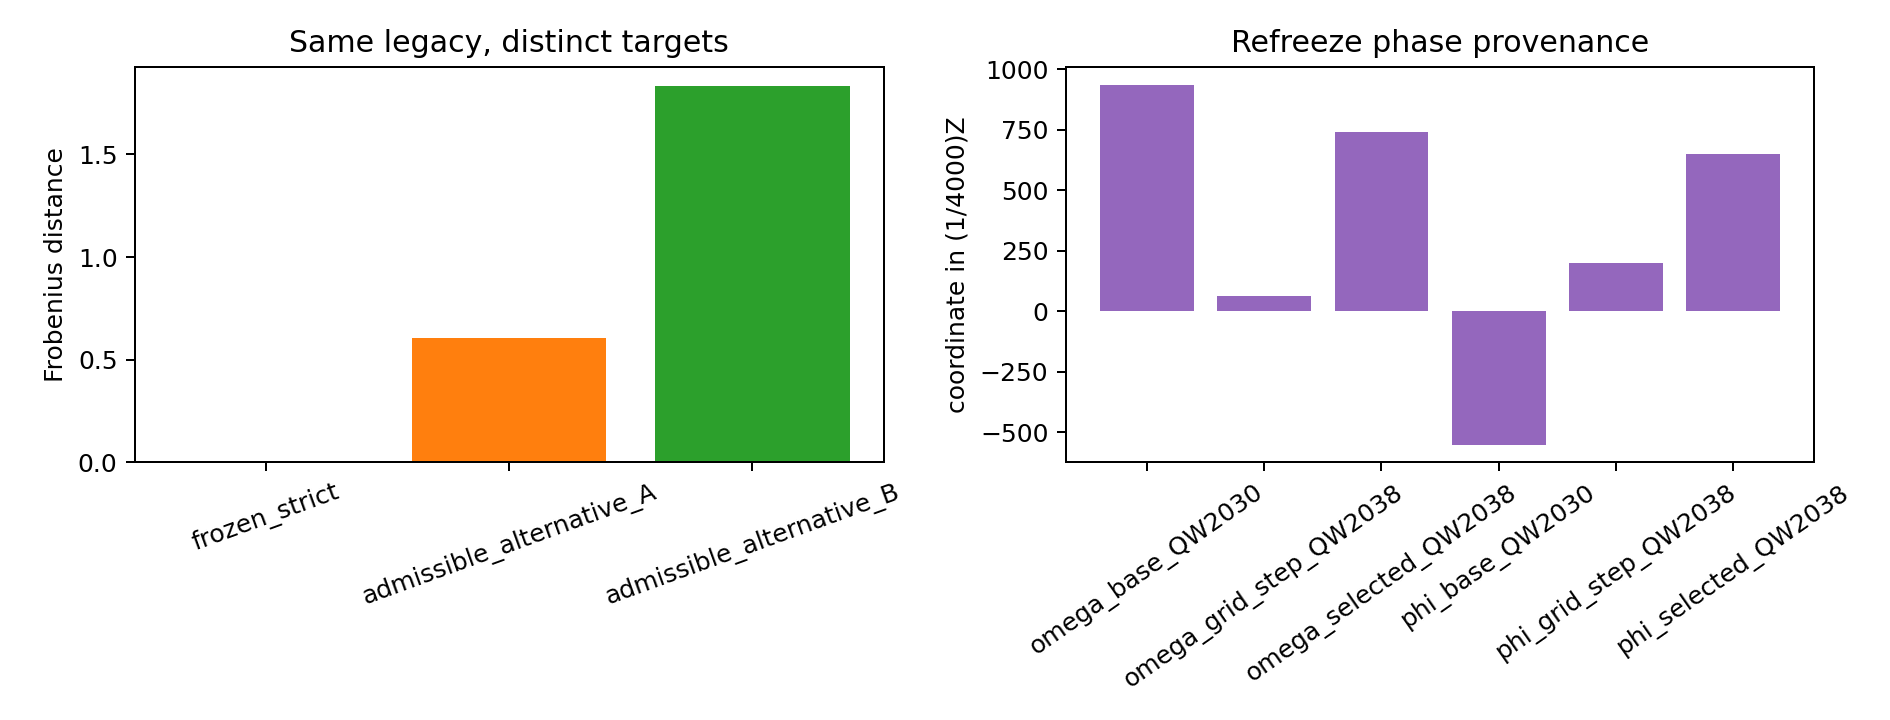
\includegraphics[width=0.97\textwidth]{FIN_Programs_323_336_Figures/p324_p325_parent_phase.png}
\caption{One legacy input with distinct target parents, and the exact QW-2030/QW-2038 phase-lattice genealogy.}
\end{figure}

\chapter{P326--P331 --- Operational and transfer programs}

\section{P326: loss-robust finite experiment}

The experiment class uses:

\begin{itemize}
\item 
all twelve vertex preparations;

\item 
a twelve-outcome vertex detector plus a no-click outcome;

\item 
mean efficiency \(0.82\) with synthetic component spread \(0.025\);

\item 
nearest-neighbor confusion near \(0.02\);

\item 
relative clock jitter with standard deviation \(0.004\);

\item 
\(48\) nuisance draws;

\item 
scale-aligned legacy dynamics.

\end{itemize}

For heat dynamics the best robust row is

\[
t=0.73863,\qquad
x=8,\qquad
\operatorname{TV}_{0.05}=0.18579,
\]

with conservative shot bound \(214\).

For wave dynamics:

\[
t=1.64532,\qquad
x=8,\qquad
\operatorname{TV}_{0.05}=0.34147,
\]

with conservative shot bound \(64\).

These are fifth-percentile detector-level distances under the supplied nuisance family.  They show that the separation found in P315 is not erased by this particular loss/\allowbreak{}confusion model.

They do not establish the nuisance family of a real detector.

\begin{figure}[htbp]
\centering
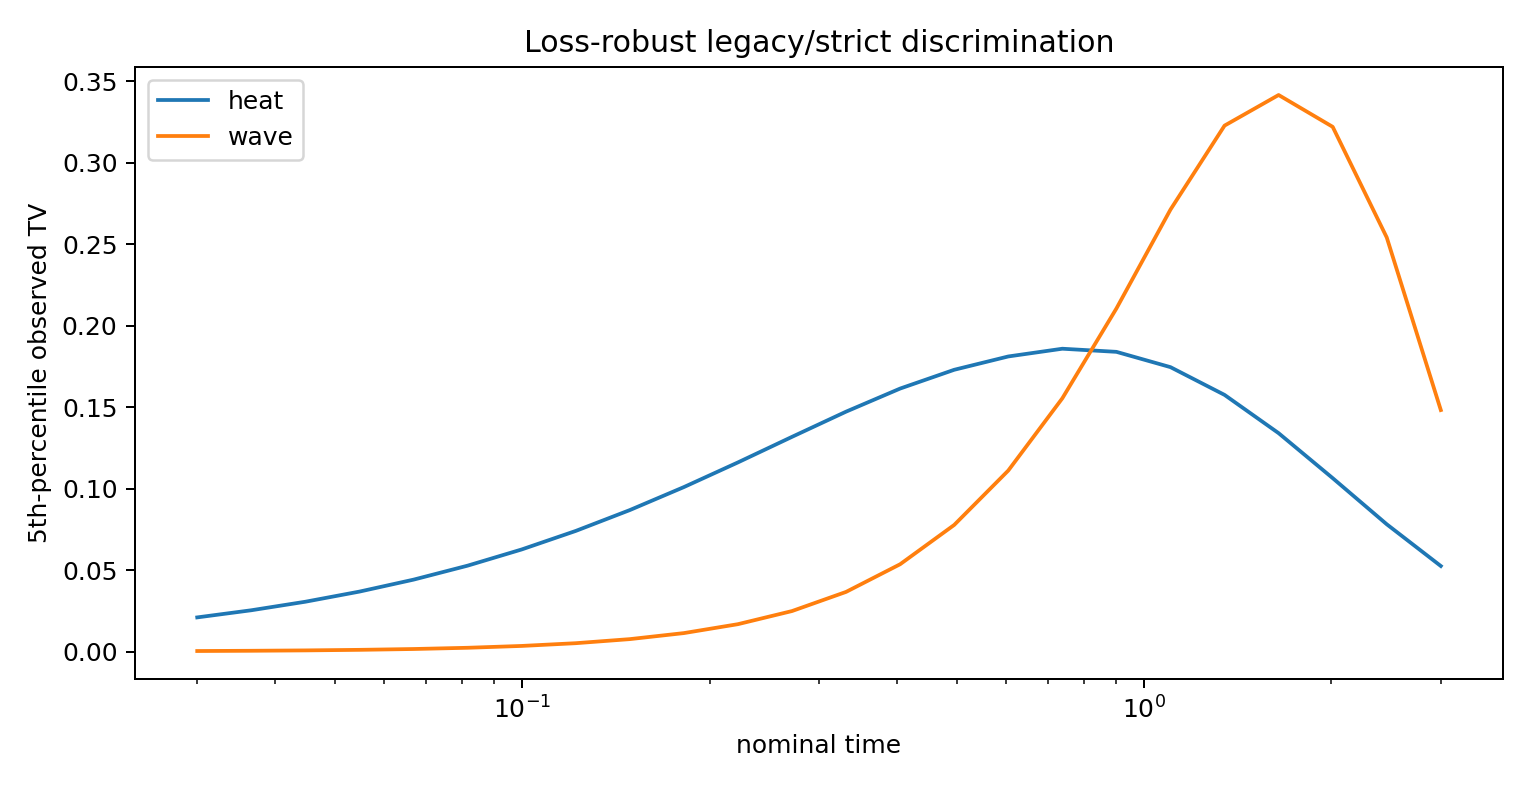
\includegraphics[width=0.97\textwidth]{FIN_Programs_323_336_Figures/p326_lossy_protocol.png}
\caption{Detector-degraded fifth-percentile operational separation under the declared synthetic nuisance model.}
\end{figure}

\section{P327: exact chamber atlas}

For positive radial weights \(w_1,\ldots,w_6\) on \(C_{12}\), the six nonzero mode values are linear:

\[
\lambda=w^{T}M,
\]

where

\[
M=
\begin{pmatrix}
2-\sqrt3&1&2&3&2+\sqrt3&4\\
1&3&4&3&1&0\\
2&4&2&0&2&4\\
3&3&0&3&3&0\\
2+\sqrt3&1&2&3&2-\sqrt3&4\\
2&0&2&0&2&0
\end{pmatrix},
\]

and

\[
\det M=-3456\sqrt3\ne0.
\]

At the uniform point \(w_0=(1/6,\ldots,1/6)\), all mode values equal \(2\). Let \(q\) be any permutation of

\[
(-5,-3,-1,1,3,5).
\]

Define

\[
c(q)=
-\frac{q_1+q_3+q_5}{3}
\]

and

\[
w(q)=
\frac16\mathbf1
+\frac1{100}
M^{-T}\bigl(q+c(q)\mathbf1\bigr).
\]

Then

\[
\sum_i w_i(q)=1,
\]

and the corresponding mode values are

\[
\lambda_i(q)=
2+\frac1{100}(q_i+c(q)).
\]

Exact enumeration over all \(720\) permutations proves:

\[
\min_{q,i}w_i(q)=\frac7{50}>0,
\]

and every adjacent mode gap is at least \(1/50\).

Thus every one of the \(720\) strict orders occurs in the interior of the positive radial simplex.  Spectral order cannot be a selector.

\begin{figure}[htbp]
\centering
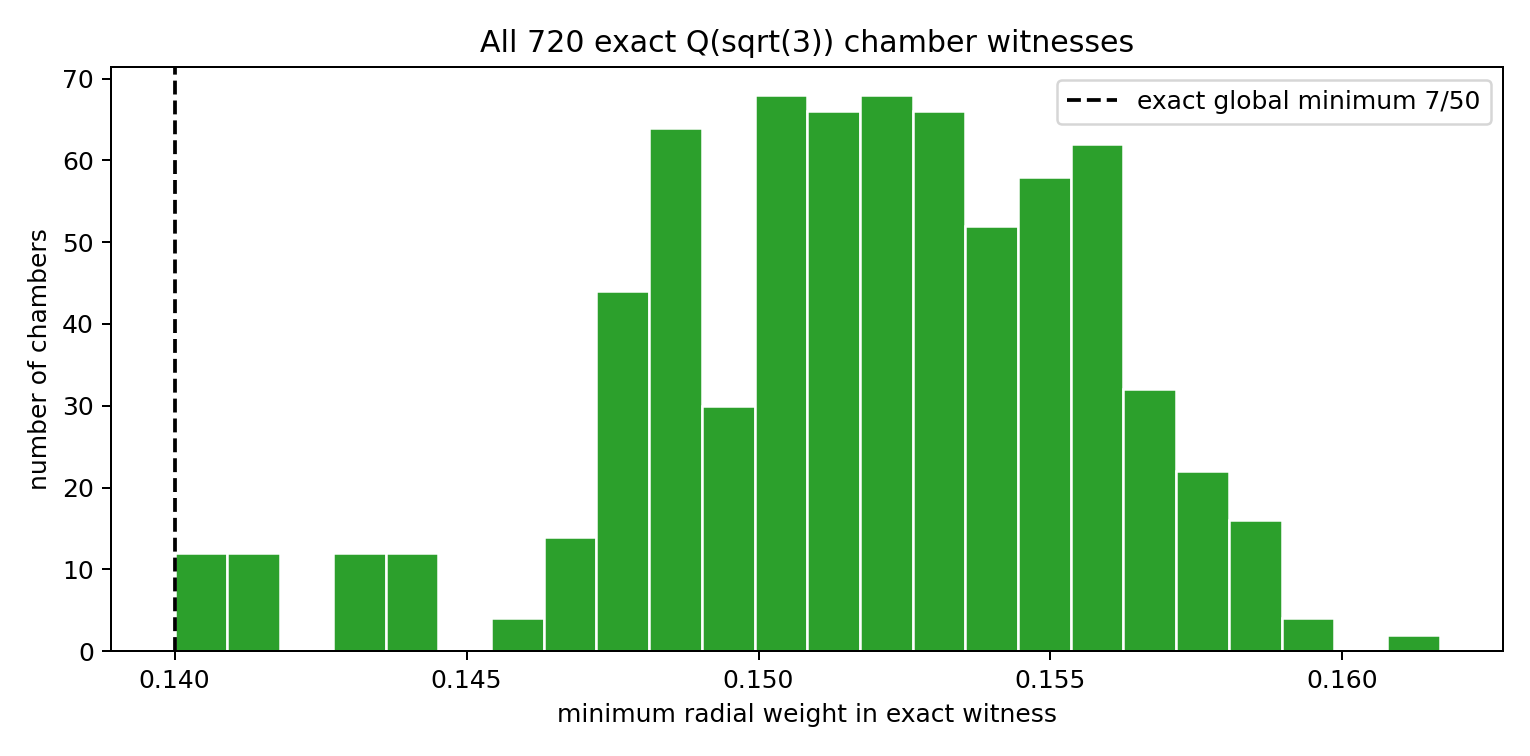
\includegraphics[width=0.97\textwidth]{FIN_Programs_323_336_Figures/p327_exact_chambers.png}
\caption{Minimum positive weights for all 720 exact algebraic spectral-order witnesses.}
\end{figure}

\section{P328: one-time wave-channel diamond distance}

For unitary channels

\[
\Phi_U(\rho)=U\rho U^\dagger,
\qquad
\Phi_V(\rho)=V\rho V^\dagger,
\]

let \(\nu\) be the distance from the origin to the convex hull of the eigenvalues of \(U^\dagger V\).  Then

\[
\frac12\|\Phi_U-\Phi_V\|_\diamond
=\sqrt{1-\nu^2}.
\]

Because the audited legacy and strict wave generators are circulant, their relative phases are simultaneously diagonalizable.  On the scanned time range the half diamond distance reaches

\[
1,
\]

with the first sampled perfect-separation time

\[
t\approx0.75591.
\]

This means that an optimal single-use quantum input and measurement can perfectly distinguish the two ideal unitary channels at that sampled time.

It does not mean that the present photonic vertex protocol realizes the optimal ancilla-assisted strategy.  A true multitime comb additionally requires interventions, memory spaces, and an SDP over declared instruments.

\section{P329: quartic-clock minimax design}

The clock family is

\[
\tau(t)=
t+a_2t^2+a_3t^3+a_4t^4,
\]

with

\[
|a_2|\le0.08,\qquad
|a_3|\le0.04,\qquad
|a_4|\le0.02,
\qquad
\tau'(0)=1.
\]

The external slope calibration removes the exact first-order degeneracy between generator scale and a free linear clock coefficient.

Among \(4368\) five-time designs, evaluated on \(27\) corner/\allowbreak{}interior clock tuples, the best design is

\[
(0.07319,\ 0.09360,\ 0.52349,\ 1.09477,\ 1.40000).
\]

Its worst-case minimum Fisher eigenvalue is

\[
7.2765\times10^{-4},
\]

which is \(3.86\) times the reference design value.

The result is minimax only for the declared quartic family and coefficient box.  Arbitrary monotone or nonparametric time warps remain capable of reopening nonidentifiability.

\begin{figure}[htbp]
\centering
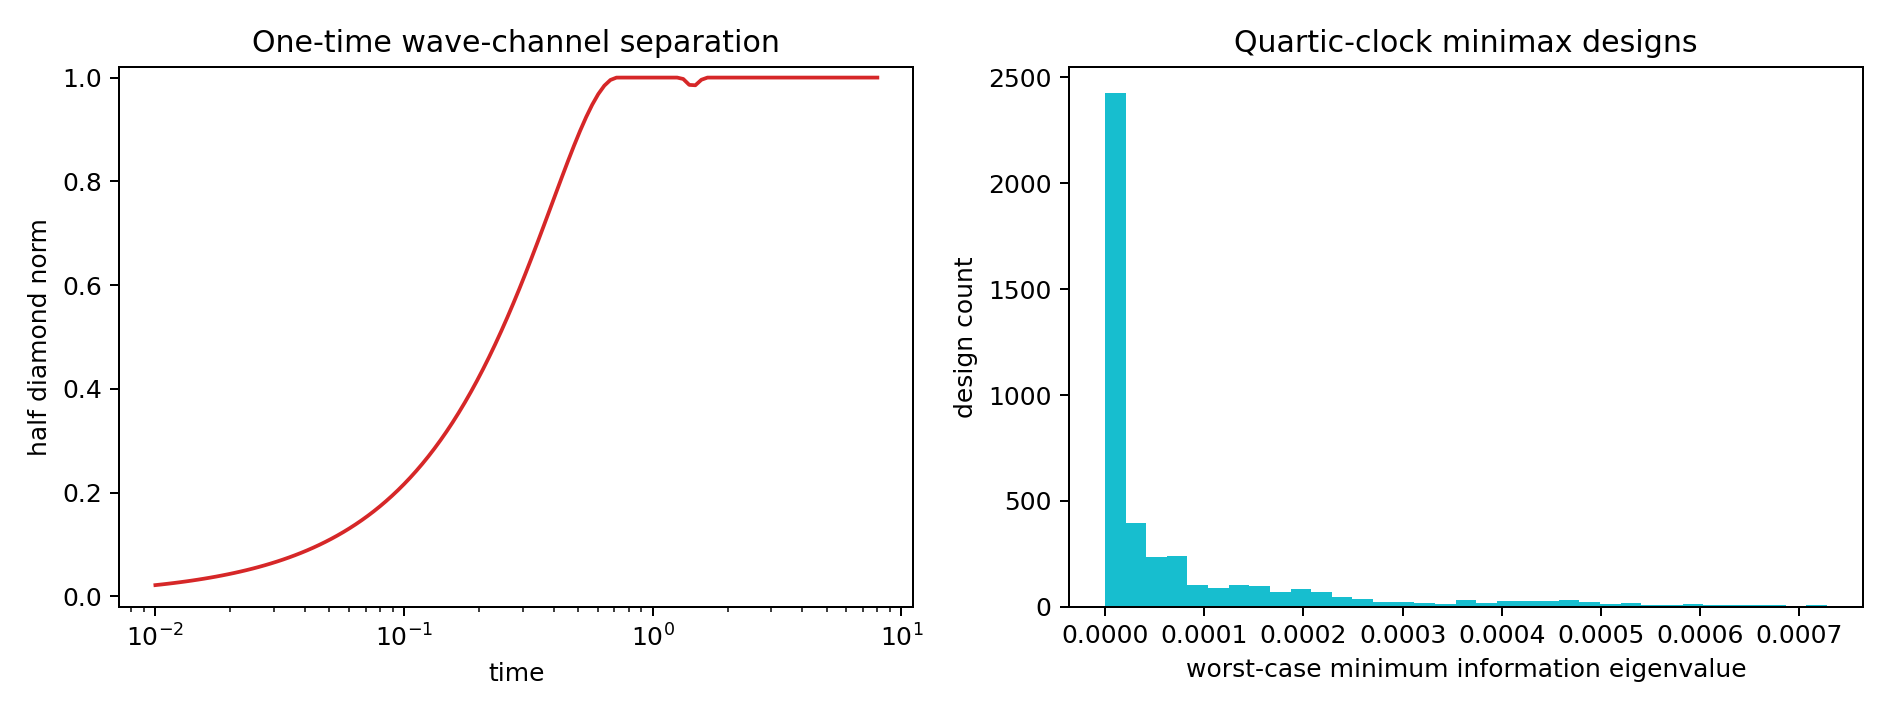
\includegraphics[width=0.97\textwidth]{FIN_Programs_323_336_Figures/p328_p329_channel_clock.png}
\caption{Ideal one-time wave-channel diamond separation and the quartic-clock minimax design distribution.}
\end{figure}

\section{P330: laboratory admission}

No manifest satisfying all of the following was admitted:

\begin{enumerate}
\item 
distinct provider, registrar, and analyst;

\item 
frozen hold-out hash;

\item 
raw event-file hash;

\item 
apparatus calibration;

\item 
non-template production status.

\end{enumerate}

Validator 241 and Pipeline 242 were therefore not run.

\section{P331: photonic transfer specification}

The best wave witness requires a dense signed \(12\)-mode coupling with nonzero coupling dynamic range approximately

\[
42.45.
\]

For witness time \(t=1.64532\), a conservative Duhamel allocation of output TV budget \(0.05\) gives generator-norm budget

\[
\|\Delta A\|
\lesssim
\frac{0.05}{t}
=0.03039.
\]

The synthetic tolerance sweep shows:

\begin{center}
\begingroup\small
\setlength{\tabcolsep}{2.5pt}
\renewcommand{\arraystretch}{1.16}
\begin{longtable}{@{}p{0.293\textwidth}p{0.335\textwidth}p{0.232\textwidth}@{}}
\toprule
\textbf{Relative coupling error SD} & \textbf{p95 output TV error} & \textbf{Pass \(0.05\) budget} \\
\midrule
\endhead
\(10^{-4}\) & \(1.25\times10^{-4}\) & yes \\
\(10^{-3}\) & \(1.16\times10^{-3}\) & yes \\
\(10^{-2}\) & \(1.19\times10^{-2}\) & yes \\
\(3\times10^{-2}\) & \(3.60\times10^{-2}\) & yes \\
\(5\times10^{-2}\) & \(5.99\times10^{-2}\) & no \\
\(10^{-1}\) & \(1.24\times10^{-1}\) & no \\
\bottomrule
\end{longtable}
\endgroup
\end{center}

The proposed implementation hypothesis is:

\begin{enumerate}
\item 
heralded single-photon source;

\item 
programmable twelve-mode interferometer;

\item 
phase and amplitude controls;

\item 
twelve SPAD/\allowbreak{}SNSPD channels with TCSPC;

\item 
independent clock and registrar;

\item 
raw event-level record.

\end{enumerate}

Because the coupling is dense and signed, a programmable interferometer or unitary dilation is more plausible than a passive nearest-neighbor waveguide array.

The pre-unblinding failure rule is mandatory: if the frozen transfer-matrix or detector hold-out exceeds its budget, reject the implementation without refitting FIN.

\begin{figure}[htbp]
\centering
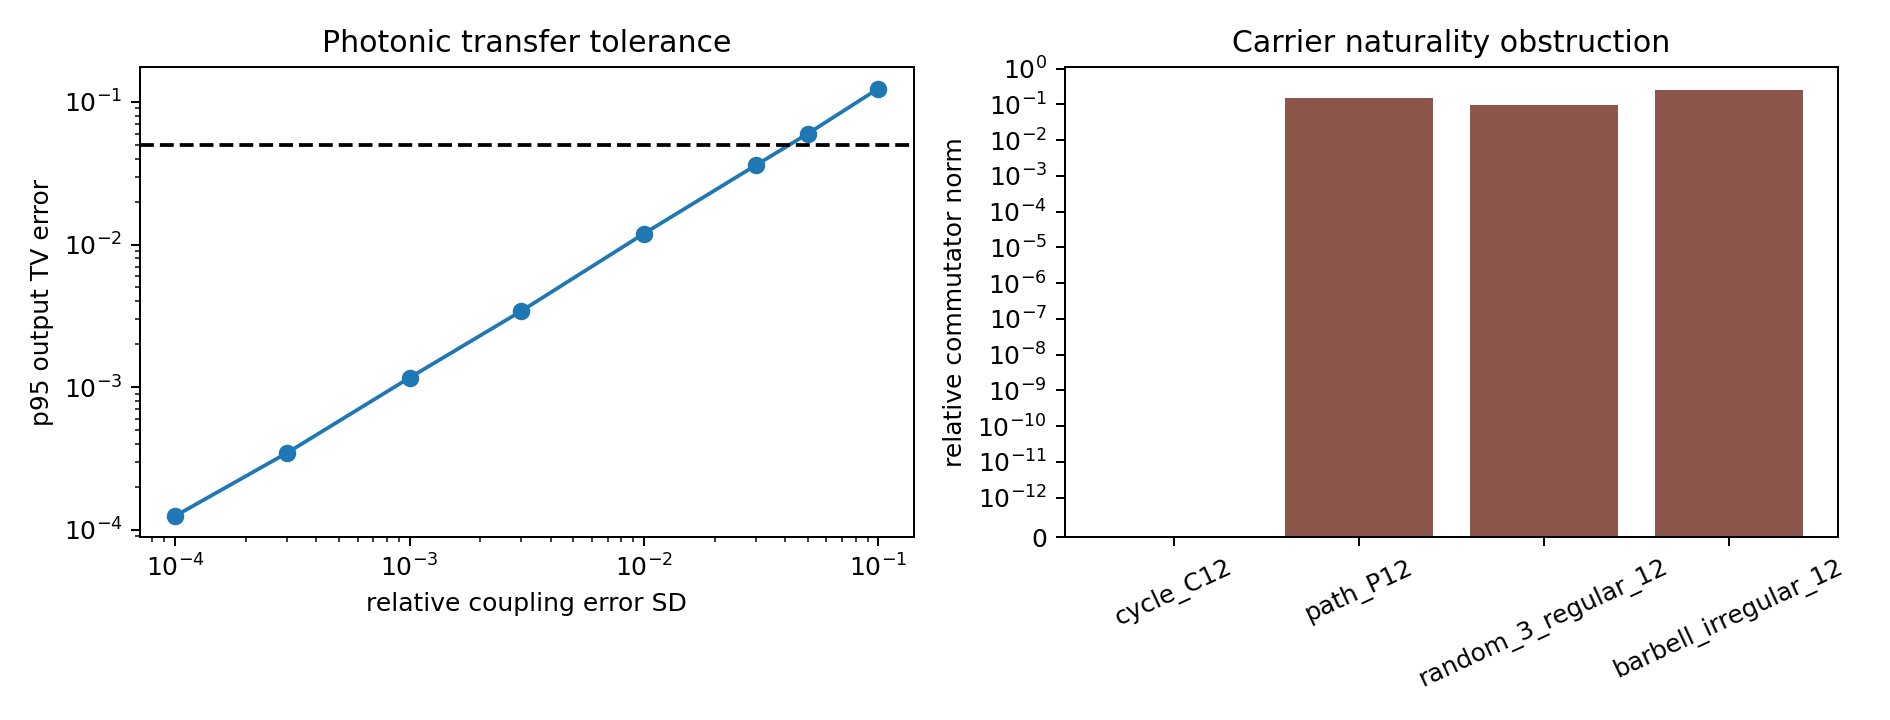
\includegraphics[width=0.97\textwidth]{FIN_Programs_323_336_Figures/p331_p333_transfer_carriers.png}
\caption{Photonic transfer tolerance and noncyclic carrier commutator obstructions.}
\end{figure}

\chapter{P332--P336 --- Interpretation, carriers, axioms, and independence}

\section{P332: signed-resource ambiguity}

The P323 signed measure can be written

\[
\sum_j u_j\delta_{r_j}
-\mathcal N_*\delta_0.
\]

At the level of scalar moments, the negative term may equally be written as

\[
\mathcal N_*e^{i\pi}\delta_0.
\]

Thus a real signed Jordan representation and a phase-\(\pi\) complex-amplitude representation give the same scalar sequence.

Other interpretations require additional structure:

\begin{center}
\begingroup\small
\setlength{\tabcolsep}{2.5pt}
\renewcommand{\arraystretch}{1.16}
\begin{longtable}{@{}p{0.281\textwidth}p{0.303\textwidth}p{0.276\textwidth}@{}}
\toprule
\textbf{Interpretation} & \textbf{Additional structure} & \textbf{Not supplied by moments} \\
\midrule
\endhead
quasiprobability & state/\allowbreak{}effect frame and free operations & operational negativity monotone \\
complex interference & phase reference and Born map & detector probability law \\
Krein space & fundamental symmetry and positive physical subspace & probability interpretation \\
open system & environment and CPTP dilation & process tensor \\
active feedback & controller, energy ledger, causal interventions & work and control record \\
\bottomrule
\end{longtable}
\endgroup
\end{center}

Therefore the signed path resource is mathematically unavoidable in its declared representation, while its physical meaning is underdetermined.

\section{P333: carrier naturality}

If

\[
A_S=f(A_L)
\]

by scalar functional calculus, then

\[
[A_L,A_S]=0.
\]

The relative commutator audit gives:

\begin{center}
\begingroup\small
\setlength{\tabcolsep}{2.5pt}
\renewcommand{\arraystretch}{1.16}
\begin{longtable}{@{}p{0.420\textwidth}p{0.420\textwidth}@{}}
\toprule
\textbf{Carrier} & \textbf{Relative commutator} \\
\midrule
\endhead
cycle \(C_{12}\) & \(5.2\times10^{-17}\) \\
path \(P_{12}\) & \(0.1482\) \\
random 3-regular graph & \(0.09356\) \\
irregular barbell graph & \(0.26046\) \\
\bottomrule
\end{longtable}
\endgroup
\end{center}

Thus scalar functional completion is not carrier-natural across the tested noncyclic family.  The cycle is special because its radial operators share a Fourier basis.

This does not exclude:

\begin{itemize}
\item 
nonscalar completion;

\item 
carrier-dependent completion;

\item 
an enlarged Hilbert space;

\item 
a target-importing joint parent.

\end{itemize}

\section{P334: minimal conditional electroweak package}

Take the historical relation only as an explicit axiom:

\[
x=
\sin^2\theta_W
=\frac{\alpha_{\mathrm{geo}}}{12}
=0.2310490602\ldots.
\]

Once the \(U(1)\) and \(SU(2)\) sectors are ordered, the coupling ratio is

\[
\frac{g'}g
=\sqrt{\frac{x}{1-x}}
=0.5481542518\ldots.
\]

The sector swap gives

\[
x\mapsto1-x,
\qquad
\frac{g'}g\mapsto\frac g{g'},
\]

so an unpointed sector pair cannot select the observed branch.

The minimal angle-only package contains:

\begin{enumerate}
\item 
one discrete sector-pointing axiom;

\item 
one role-law axiom \(x=\alpha_{\mathrm{geo}}/12\);

\item 
zero new continuous parameters for the angle alone.

\end{enumerate}

A minimal tree-level mass scaffold additionally needs at least:

\begin{enumerate}
\item 
an overall gauge coupling \(g\);

\item 
a symmetry-breaking scale \(v\);

\item 
representation and covariant-derivative laws;

\item 
a symmetry-breaking sector;

\item 
a mass/\allowbreak{}observable map.

\end{enumerate}

No full electroweak theory follows from the current spectrum.

\section{P335: independence cube}

Let the resource vector be

\[
R=(N,\Phi,C,P,S)
\in\{0,1\}^5,
\]

where:

\begin{itemize}
\item 
\(N\): signed path resource;

\item 
\(\Phi\): nontorsion phase;

\item 
\(C\): independent cross law;

\item 
\(P\): pointing;

\item 
\(S\): dimensional scale.

\end{itemize}

All \(2^5=32\) product-signature models were constructed.  For each resource, there exists a model in which the other four are present and that resource is absent:

\[
01111,\quad
10111,\quad
11011,\quad
11101,\quad
11110.
\]

Therefore no implication

\[
R_i
\Leftarrow
\bigwedge_{j\ne i}R_j
\]

is valid in the minimal uncoupled signature.

This result is formalized in Lean 4.28.  It proves logical independence before coupling laws are added.  It does not prove that a future FIN dynamical law cannot co-generate several resources.

\begin{figure}[htbp]
\centering
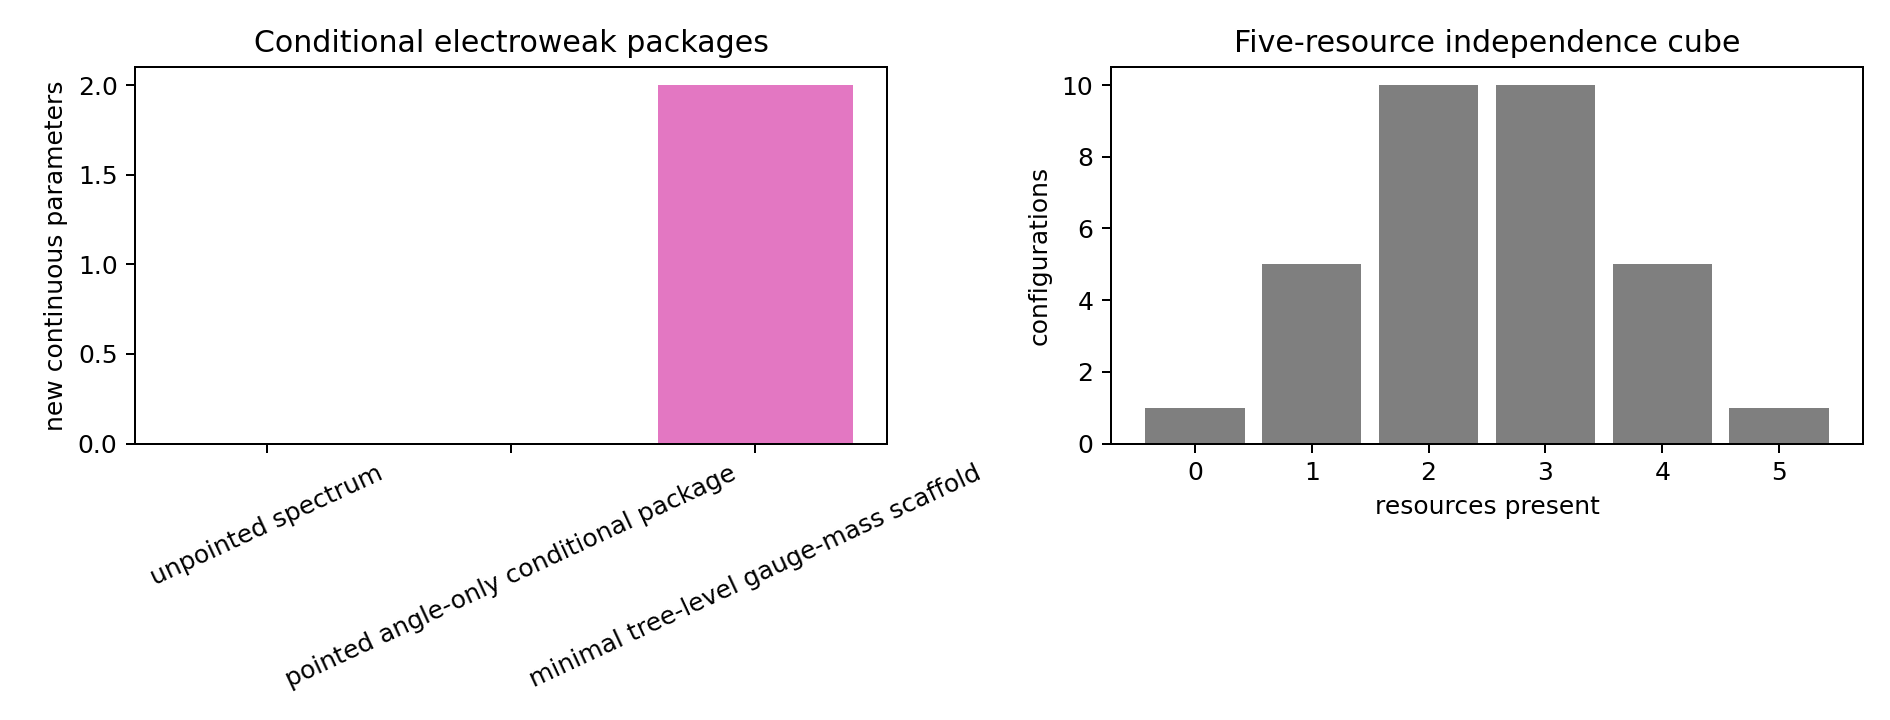
\includegraphics[width=0.97\textwidth]{FIN_Programs_323_336_Figures/p334_p335_axioms_independence.png}
\caption{Conditional electroweak parameter accounting and the five-resource independence cube.}
\end{figure}

\section{P336: reservoir gate}

No package contains certified:

\begin{itemize}
\item 
physical hardware data;

\item 
paired controls and matched seeds;

\item 
frozen primary endpoint;

\item 
calibration record;

\item 
independent custody.

\end{itemize}

The external reservoir experiment remains blocked.

\chapter{Cross-program synthesis}

\section{The refined bridge-resource diagram}

\[
\begin{array}{c}
K_{\mathrm{legacy}}
\\[1mm]
\downarrow\quad
\text{source-independent completion fiber}
\\[1mm]
\boxed{\text{missing selector/cross law}}
\\[1mm]
\downarrow
\\[1mm]
\text{signed attenuation completion}
\quad+\quad
\text{refreeze phase lattice}
\\[1mm]
\downarrow
\\[1mm]
K_{\mathrm{strict}}
\quad\text{as a frozen operational target}
\\[1mm]
\downarrow
\\[1mm]
\text{clock + scale + preparation + instrument + record}
\\[1mm]
\downarrow
\\[1mm]
\text{falsifiable physical experiment}
\end{array}
\]

The diagram contains two different notions of "generation":

\begin{enumerate}
\item 
mathematical construction after target data are supplied;

\item 
source-independent derivation before the target is known.

\end{enumerate}

Current FIN has strong examples of the first and open obligations for the second.

\section{A smaller object does not yet replace the resource tuple}

P335 shows that no one resource follows logically from the other four in the minimal signature.  Consequently, replacing the five-component budget by one unnamed "deeper object" would currently hide assumptions rather than reduce them.

A legitimate smaller object must arrive with coupling theorems proving that its projections generate:

\[
(N,\Phi,C,P,S).
\]

No such theorem is currently exported.

\section{What the phase result means}

P325 changes the interpretation of O66 from Release 10.28.

The phase generator \(e^{i/4000}\):

\begin{itemize}
\item 
is exactly minimal for the frozen rational tuple;

\item 
is exactly minimal for the QW-2030/\allowbreak{}QW-2038 scan lattice;

\item 
is not contained in the finite legacy phase group;

\item 
is procedurally generated by the refreeze design;

\item 
is not yet internally generated by strict informational dynamics.

\end{itemize}

This is a sharper and more informative result than calling \(1/4000\) an arbitrary fitted decimal.  It also prevents promoting a procedural grid unit into an ontological constant.

\section{Operational consequences}

Three different distance levels are now available:

\begin{enumerate}
\item 
vertex-measurement TV distance;

\item 
detector-degraded robust TV distance;

\item 
ideal one-time quantum-channel diamond distance.

\end{enumerate}

They answer different questions and must not be conflated.  In particular, the ideal diamond distance reaching one does not eliminate the need to compile and calibrate the corresponding optimal input and measurement.

\chapter{Failed approaches and no-go boundaries}

\begin{center}
\begingroup\small
\setlength{\tabcolsep}{2.5pt}
\renewcommand{\arraystretch}{1.16}
\begin{longtable}{@{}p{0.339\textwidth}p{0.209\textwidth}p{0.312\textwidth}@{}}
\toprule
\textbf{Candidate} & \textbf{Verdict} & \textbf{Reason} \\
\midrule
\endhead
the \(0.4067\) negativity was only a grid artifact & Refuted & matching continuum primal--dual certificate \\
\(1/4000\) is presently an internal FIN constant & Refuted on current provenance & it is the gcd unit of supplied scan centers and steps \\
a common parent generates strict automatically & Refuted & cross block reads the chosen target \\
spectral order selects strict & Refuted exactly & all \(720\) orders have positive algebraic witnesses \\
detector loss erases all legacy/\allowbreak{}strict difference & Refuted in supplied nuisance class & robust TV remains \(0.186/0.341\) \\
one-time ideal wave channels are operationally equivalent & Refuted & half diamond norm reaches one \\
clock design alone fixes an uncalibrated linear clock & Refuted & scale and clock-slope columns coincide \\
signed mass uniquely means quantum interference & Refuted & several inequivalent realizations share the moments \\
cyclic scalar completion is carrier-universal & Refuted in tested family & three noncyclic commutators are nonzero \\
unpointed spectrum gives the electroweak branch & Refuted & sector swap sends \(x\) to \(1-x\) \\
four bridge resources imply the fifth & Refuted in minimal signature & five single-omission models \\
repository output supplies external experiment & Blocked & custody, calibration, raw data, hold-out absent \\
\bottomrule
\end{longtable}
\endgroup
\end{center}

\chapter{Recommended Programs P337--P350}

Probabilities estimate the chance of a decisive result, including a rigorous negative result.

\begin{center}
\begingroup\fontsize{7}{8.4}\selectfont
\setlength{\tabcolsep}{2.5pt}
\renewcommand{\arraystretch}{1.16}
\begin{longtable}{@{}p{0.055\textwidth}p{0.088\textwidth}p{0.266\textwidth}p{0.312\textwidth}p{0.139\textwidth}@{}}
\toprule
\textbf{Rank} & \textbf{Program} & \textbf{Study} & \textbf{Decisive output} & \textbf{Probability} \\
\midrule
\endhead
1 & P337 & formal algebraic/\allowbreak{}interval P323 certificate & machine-check node, weight, and dual-feasibility enclosures & 0.91 \\
2 & P338 & full oscillatory-kernel signed resource & extend the moment extremizer from attenuation to the complete signed strict kernel & 0.84 \\
3 & P339 & continuous refreeze sensitivity audit & distinguish stable objective basin from grid-coordinate artifact on frozen hold-out & 0.88 \\
4 & P340 & natural common-parent theorem & classify carrier-natural transformations across cycles, paths, and irregular graphs & 0.82 \\
5 & P341 & compiled photonic inverse calibration & convert the P331 matrix budget into a mesh and calibration-inversion executable & 0.83 \\
6 & P342 & independent P241 production run & admit, validate, hash, and execute one real event bundle & 0.28 \\
7 & P343 & multitime quantum-comb SDP & compute an adaptive operational distance for declared interventions & 0.76 \\
8 & P344 & nonparametric clock bounds & replace the quartic box by monotone Sobolev or spline uncertainty & 0.79 \\
9 & P345 & carrier-universal strict invariants & identify which phase/\allowbreak{}compression features survive graph changes naturally & 0.75 \\
10 & P346 & bridge-resource monotones & define free completion maps and monotones for negativity, phase, pointing, and scale & 0.74 \\
11 & P347 & resource coupling theorem search & test whether one strict law can co-generate two or more O86 factors & 0.68 \\
12 & P348 & falsifiable conditional EW package & preregister observables that are not algebraic restatements of the angle axiom & 0.72 \\
13 & P349 & dimensional conversion metrology & specify operational calibration of \(\hbar_*,\ell_*,\tau_*\) without calling them emergent & 0.70 \\
14 & P350 & external reservoir execution & run paired hardware and control records under a frozen endpoint & 0.25 \\
\bottomrule
\end{longtable}
\endgroup
\end{center}

\section{Recommended immediate sequence}

\[
\boxed{
P337
\longrightarrow
P338
\longrightarrow
P339
\longrightarrow
P340
\longrightarrow
P341
\longrightarrow
P343
}
\]

The sequence first upgrades the strongest new mathematical result, then includes the oscillatory phase, audits the actual selection procedure, demands carrier naturality, compiles a physical transfer design, and finally constructs the correct multitime operational distance.

P342 and P350 remain external and cannot be completed by repository simulation.

\chapter{Research roadmap}

\section{Mathematical track}

The highest-value mathematical tasks are:

\begin{enumerate}
\item 
formalize the P323 extremal certificate;

\item 
determine the signed resource of the full kernel, not only its envelope;

\item 
classify natural parent transformations;

\item 
define resource monotones and coupling laws.

\end{enumerate}

Success may be either a constructive theorem or a no-go theorem.

\section{Operational track}

The operational track should:

\begin{enumerate}
\item 
compile the strict unitary into a declared optical architecture;

\item 
invert calibration records into a confidence set for the implemented channel;

\item 
freeze preparation, time, measurement, and failure thresholds;

\item 
keep provider, registrar, and analyst separate;

\item 
report a failed calibration or null result without model repair.

\end{enumerate}

\section{Conditional-physics track}

Conditional packages may be developed, but each supplied object must remain visible:

\[
\text{informational core}
+\text{conversion axioms}
+\text{sector axioms}
+\text{apparatus model}.
\]

No conditional theorem is to be renamed a strict zero-parameter prediction.

\chapter{Limitations}

\begin{enumerate}
\item 
The P323 theorem is analytic, while the displayed FIN evaluation is a 90-digit computation rather than a fully checked algebraic-number proof.

\item 
P324 alternatives demonstrate underdetermination; they are not claimed as physical competitors.

\item 
P325 proves procedural phase provenance, not causal physical origin.

\item 
P326, P329, and P331 use synthetic nuisance families.

\item 
P327 classifies order only, not spectral magnitude or physical likelihood.

\item 
P328 treats ideal one-use unitary wave channels, not a full comb.

\item 
P333 tests four carriers and one necessary scalar-calculus condition.

\item 
P334 is explicitly axiom-augmented.

\item 
P335 proves independence only before additional coupling laws.

\item 
P330 and P336 remain externally blocked.

\end{enumerate}

\chapter{Final conclusion}

The deepest result of this round is not that another physical role has been found.  It is that three previously blurred issues have been separated exactly.

The strict attenuation has a quantitatively exact signed-moment resource:

\[
\mathcal N_{\mathrm{path}}^{\min}
=0.406706334692258\ldots.
\]

The frozen strict phase has an exact procedural lattice source:

\[
\frac1{4000}\mathbb Z,
\]

generated by the QW-2030 center and QW-2038 scan increments.

And the remaining bridge resources are not consequences of one another in the minimal uncoupled signature.

Therefore the current scientifically surviving interpretation is:

\begin{quote}\itshape
FIN contains a mathematically coherent informational operator target with exact spectral, moment, phase-lattice, and operational certificates.  Its legacy-to-strict completion and its transition to physics require separately declared source, sector, scale, instrument, and record structures.  Some of those structures can be constructed conditionally; none has yet been shown to emerge as one unavoidable strict physical law.

\end{quote}

This is stronger than an interpolation claim and weaker than a physical theory.  It is the correct boundary for the next research round.

\chapter{References}

\begin{enumerate}
\item 
N. I. Akhiezer, \emph{The Classical Moment Problem}, Oliver \& Boyd, 1965.

\item 
S. Karlin and W. J. Studden, \emph{Tchebycheff Systems: With Applications in Analysis and Statistics}, Wiley, 1966.

\item 
M. G. Krein and A. A. Nudelman, \emph{The Markov Moment Problem and Extremal Problems}, American Mathematical Society, 1977.

\item 
R. Bhatia, \emph{Matrix Analysis}, Springer, 1997.

\item 
T. Kato, \emph{Perturbation Theory for Linear Operators}, Springer, 1995.

\item 
M. A. Nielsen and I. L. Chuang, \emph{Quantum Computation and Quantum Information}, Cambridge University Press, 2010.

\item 
J. Watrous, \emph{The Theory of Quantum Information}, Cambridge University Press, 2018.

\item 
G. Gutoski and J. Watrous, "Toward a General Theory of Quantum Games," Proceedings of STOC, 2007.

\item 
M. Reed and B. Simon, \emph{Methods of Modern Mathematical Physics I: Functional Analysis}, Academic Press, 1980.

\item 
Existing FIN repository packets K1, K2, F2, F3, S2, QW-2030, QW-2038, QW-2049, P295--P322, and the Release 10.28 executable artifacts.

\end{enumerate}


\clearpage
\chapter*{Reproduction certificate}
\addcontentsline{toc}{chapter}{Reproduction certificate}
\begin{Verbatim}[fontsize=\small]
MPLCONFIGDIR=/tmp/mpl-fin \
python3 -m unittest -v test_fin_programs_323_336.py
\end{Verbatim}
Expected result: 18 tests passed, 0 failed.  The suite recompiles the
dependency-free Lean 4.28 source.  Detector, clock, coupling-error, and
finite-count assumptions are synthetic.  P330 and P336 admit no external
laboratory or hardware evidence.

\medskip
\noindent\textbf{Suggested citation:}

\.Zuchowski, K. (2026). \emph{FIN Research Programs P323--P336:
Exact Resource Certificates, Refreeze Provenance, and Operational Transfer
Boundaries} (Release 10.29; Version 1.0.0) [Preprint]. Zenodo.

\end{document}
